\documentclass{beamer}[9pt]
\usetheme{Madrid}

\title{Presentation \#2}

\author{Andre Sealy, Federica Malamisura, Swapnil Pant}
\institute{Stevens Institute of Technology}
\date{May 5, 2025}

\usepackage{graphicx}
\usepackage{booktabs}
\usepackage{amsmath}
\usepackage{tabularx}

\begin{document}
	
	% Title Slide
	\frame{\titlepage}
	
	% Overview
	\begin{frame}{Overview}
		\begin{itemize}
			\item Analyze high-volatility equities in the Technology sector.
			\item Apply time series techniques (ARIMA, VAR, and GARCH) to uncover dynamics in returns, volatility clustering, and interdependencies across stocks.
			\item Quantify downside risk using Historical, Parametric, and GARCH-based Value-at-Risk (VaR) measures; extend to Expected Shortfall for deeper tail-risk insights.
		\end{itemize}
	\end{frame}
	

% Cumulative Returns Figure
\begin{frame}{Vector Autoregressive Models}
	\begin{figure}{Cumulative Returns}
		\centering
		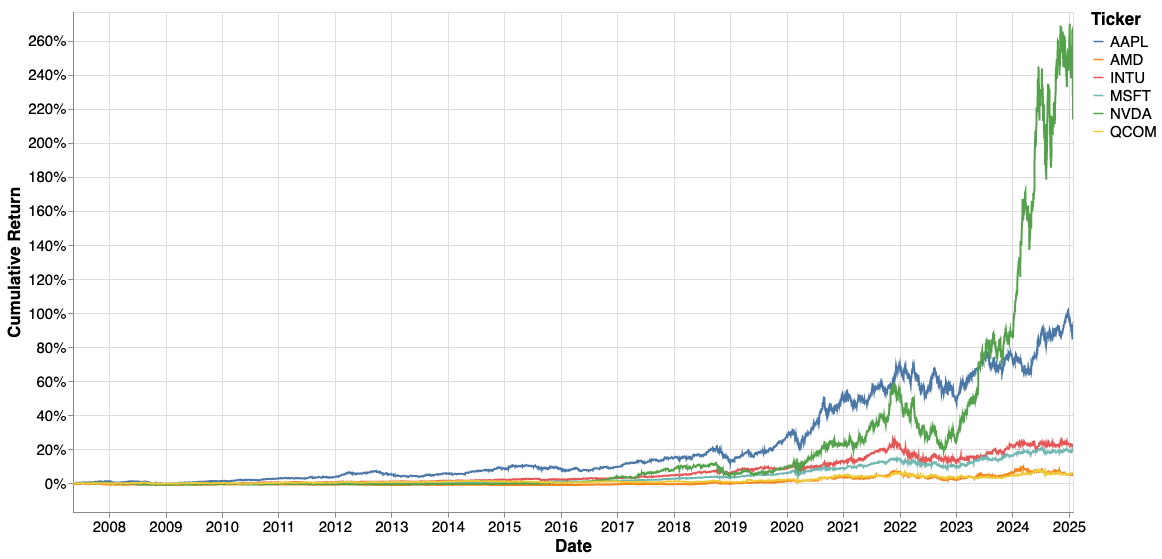
\includegraphics[width=0.9\textwidth]{plots/sample_stocks.png} % Replace with actual extracted figure
		\caption{Cumulative Returns for Sample Securities}
	\end{figure}
\end{frame}

% Descriptive Statistics Table (Example)
\begin{frame}{Vector Autoregressive Models}
	\begin{figure}[!h]
		\centering
		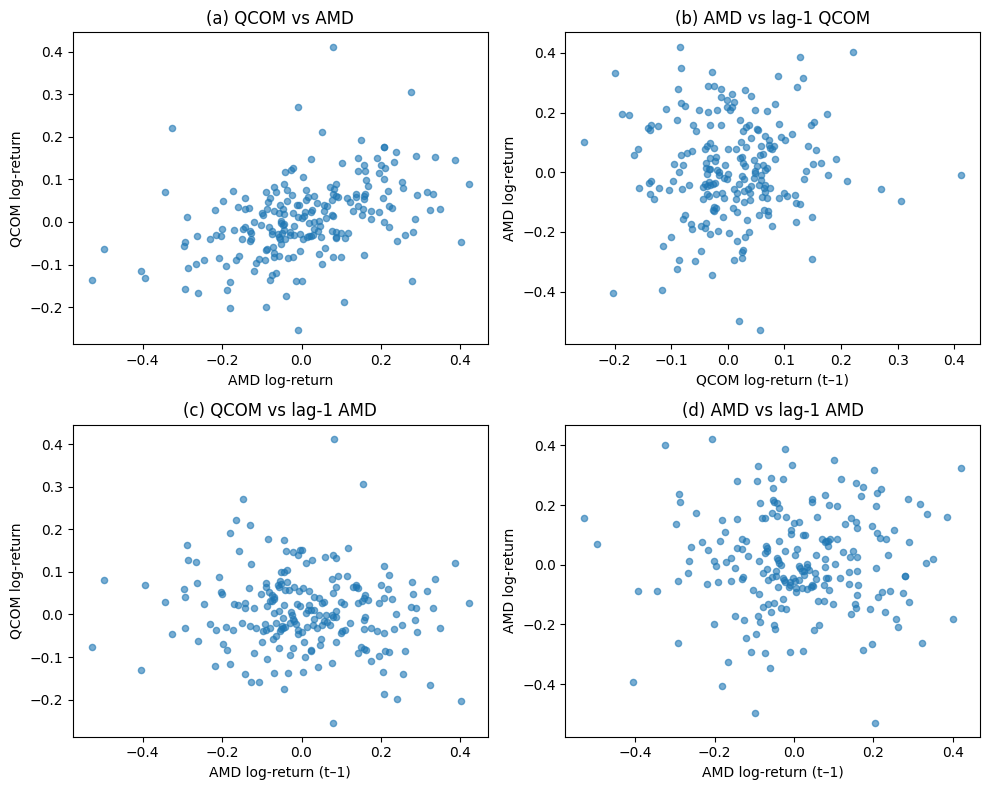
\includegraphics[width=0.8\linewidth]{plots/amd_qcom_scatter.png}
		\caption{Scatter Plot of Monthly log returns of AMD and QCOM}
		\label{fig:amd_qcom_scatter}
	\end{figure}
\end{frame}

\begin{frame}{Vector Autoregressive Models}
	\begin{figure}[!h]
		\centering
		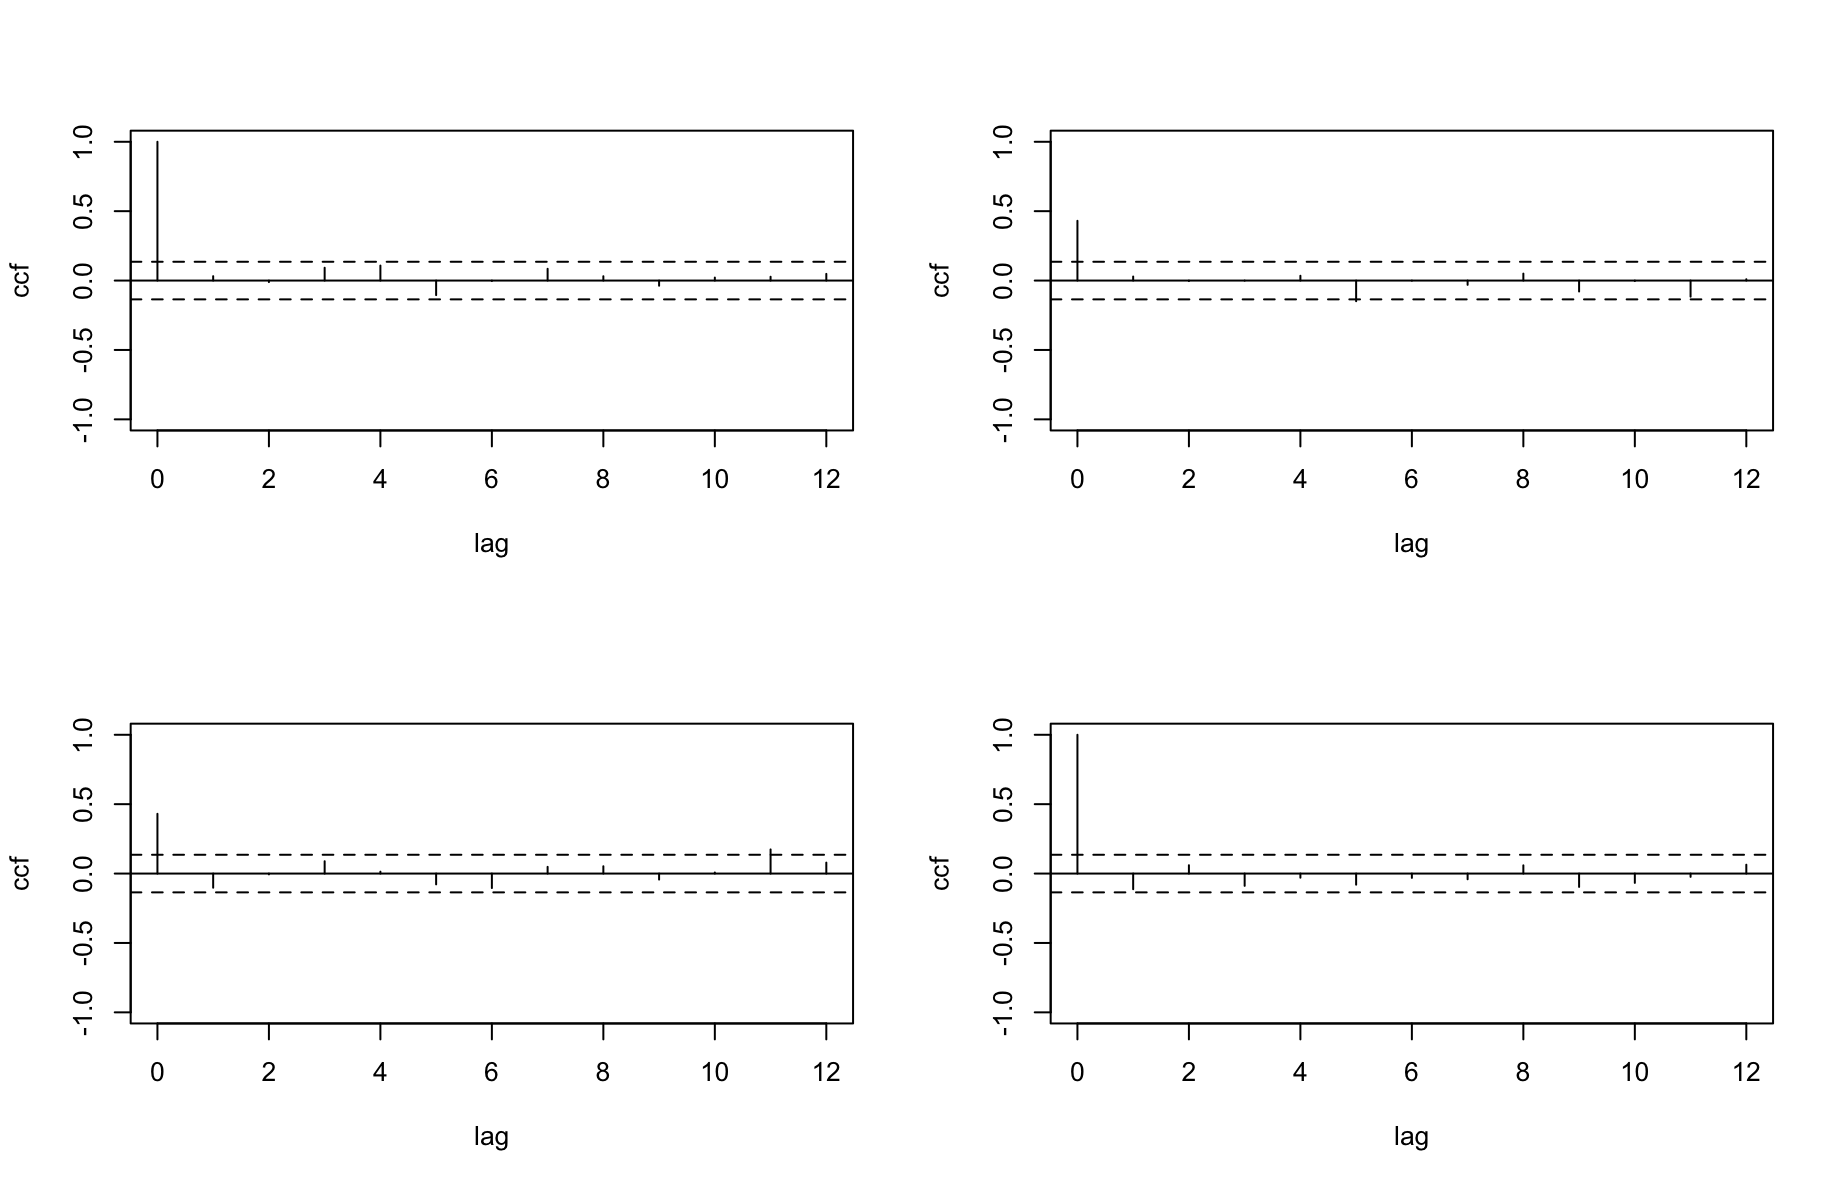
\includegraphics[width=0.8\linewidth]{plots/ccf_qcom_amd.png}
		\caption{(Top Left: ACF of QCOM; Top Right: Cross Correlation between QCOM and AMD; Bottom Left: ACF of AMD; Bottom Right: Cross Correlation between AMD and QCOM}
		\label{fig:ccf_qcom_amd}
	\end{figure}
\end{frame}
	
\begin{frame}{Vector Autoregressive Models}
\scriptsize
\begin{table}[ht]
	\centering
	\caption{Lag Length Selection Criteria from \texttt{VARselect}}
	\begin{tabular}{lcccccc}
		\toprule
		& \textbf{1} & \textbf{2} & \textbf{3} & \textbf{4} & \textbf{5} & \textbf{6} \\
		\midrule
		AIC(n)  & 13.61680 & 13.65035 & 13.65723 & 13.67909 & 13.68640 & 13.70674 \\
		HQ(n)   & 13.65600 & 13.71568 & 13.74870 & 13.79669 & 13.83014 & 13.87662 \\
		SC(n)   & 13.71373 & 13.81189 & 13.88340 & 13.96987 & 14.04180 & 14.12677 \\
		FPE(n)  & 819792.47 & 847769.53 & 853653.93 & 872568.81 & 879055.56 & 897241.50 \\
		\midrule
	\end{tabular}
	
	\vspace{0.5em}
	
	\begin{tabular}{lcccccc}
		\toprule
		& \textbf{7} & \textbf{8} & \textbf{9} & \textbf{10} & \textbf{11} & \textbf{12} \\
		\midrule
		AIC(n)  & 13.73149 & 13.76261 & 13.79238 & 13.81291 & 13.78931 & 13.81530 \\
		HQ(n)   & 13.92749 & 13.98475 & 14.04065 & 14.08732 & 14.08985 & 14.14198 \\
		SC(n)   & 14.21613 & 14.31187 & 14.40626 & 14.49141 & 14.53243 & 14.62304 \\
		FPE(n)  & 919886.57 & 949190.04 & 978160.34 & 998822.64 & 975964.07 & 1002200.00 \\
		\bottomrule
	\end{tabular}
	\label{tab:varselect-split}
\end{table}
\end{frame}

\begin{frame}{Vector Autoregressive Models}
Our Var(1) model for two series can be represented in the following form:
\[
	\begin{bmatrix}
	\text{QCOM}_t \\
	\text{AMD}_t
\end{bmatrix}
=
\begin{bmatrix}
	2.1352 \\
	1.9618
\end{bmatrix}
+
\begin{bmatrix}
	0.02356 & 0.03490 \\
	-0.03611 & -0.08491
\end{bmatrix}
\begin{bmatrix}
	\text{QCOM}_{t-1} \\
	\text{AMD}_{t-1}
\end{bmatrix}
+
\begin{bmatrix}
	\epsilon_{\text{QCOM},t} \\
	\epsilon_{\text{AMD},t}
\end{bmatrix}
\]
which can then be rewritten as:
	\[
		\begin{aligned}
		\text{QCOM}_t=0.002356\cdot\text{QCOM}_{t-1}+0.03490\cdot\text{AMD}_{t-1}+2.1352\\
		\text{AMD}_t=-0.03611\cdot\text{QCOM}_{t-1}-0.08491\cdot\text{AMD}_{t-1}+1.9618\\
	\end{aligned}
	\]
\end{frame}
\begin{frame}
\frametitle{Cointegration}

\centering
{\Large Cointegration}
\end{frame}



\begin{frame}{Cointegration}

	The augmented Engle-Granger cointegration test evaluates whether two or more non-stationary time series share a long-term equilibrium relationship.
\end{frame}

\begin{frame}{Cointegration}
	\textbf{Hypothesis Test Structure}
	\begin{itemize}
		\item $H_0$: No cointegration exists between the time series.
		\item $H_a$: Residuals are stationary.
	\end{itemize}

	\textbf{Test Producer}
	\begin{enumerate}
		\item Regress one $I(1)$ variable $y_t$ on the other $I(1)$ variables $(x_t)$:
		\[
			y_t=\beta_0+\beta_1 x_t+u_t
		\]
		\item Test $\hat{u}$ for stationarity using 
		\[
			\Delta\hat{u} t=\alpha\hat{u} t-1+\sum i=1^{p}\Delta\hat{u}_{t-1}+\epsilon_t
		\]
		where the test statistic is the t-ratio for $\alpha$
	\end{enumerate}
\end{frame}

\begin{frame}{Cointegration}
	\begin{figure}[!h]
		\centering
		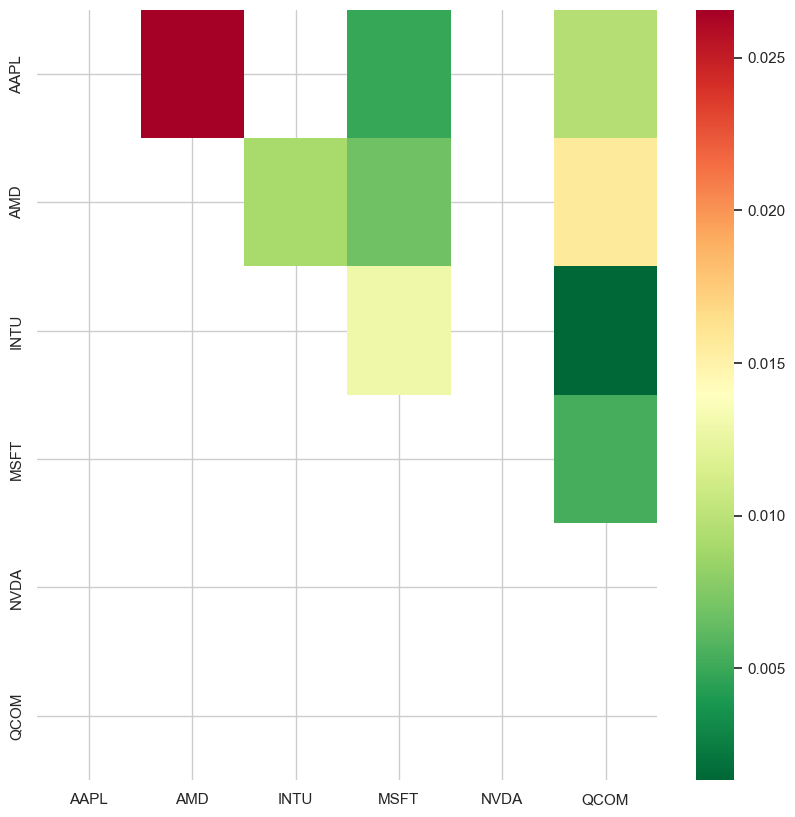
\includegraphics[width=0.55\linewidth]{plots/engle_granger.png}
		\caption{Cointegration Pairs based on Engle-Granger}
	\end{figure}
\end{frame}

\begin{frame}{Cointegration}
	\begin{figure}[!h]
		\centering
		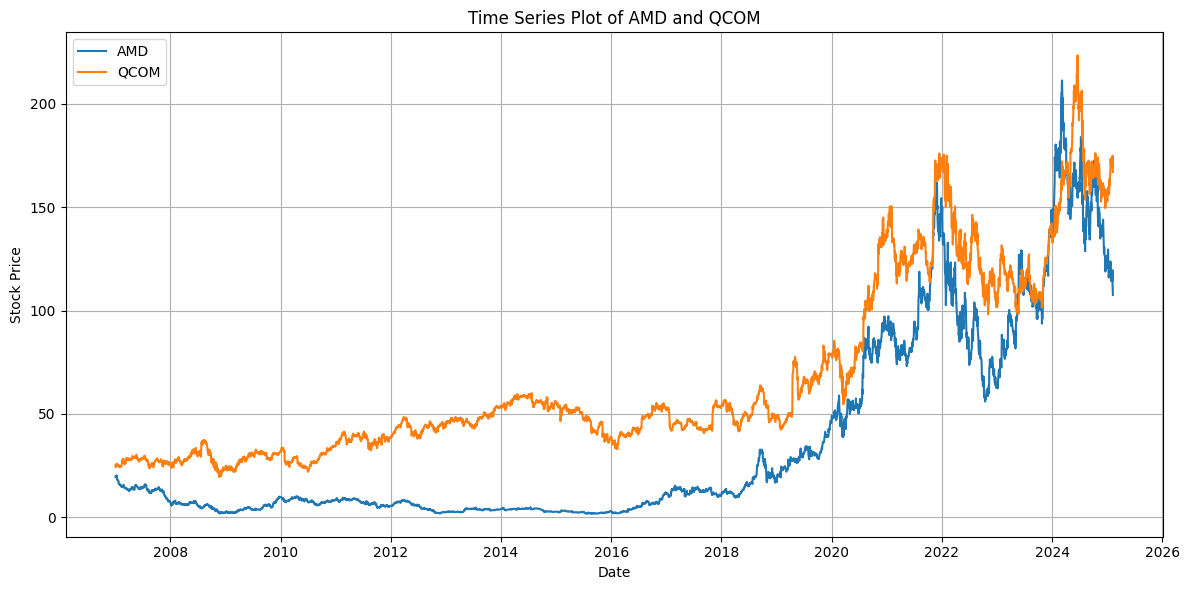
\includegraphics[width=0.8\linewidth]{plots/QCOM_AMD.png}
		\caption{Cumulative Returns of QCOM and AMD}
		\label{fig:qcom_amd_cumulative}
	\end{figure}
\end{frame}

\begin{frame}{Cointegration}
	\begin{figure}[!h]
		\centering
		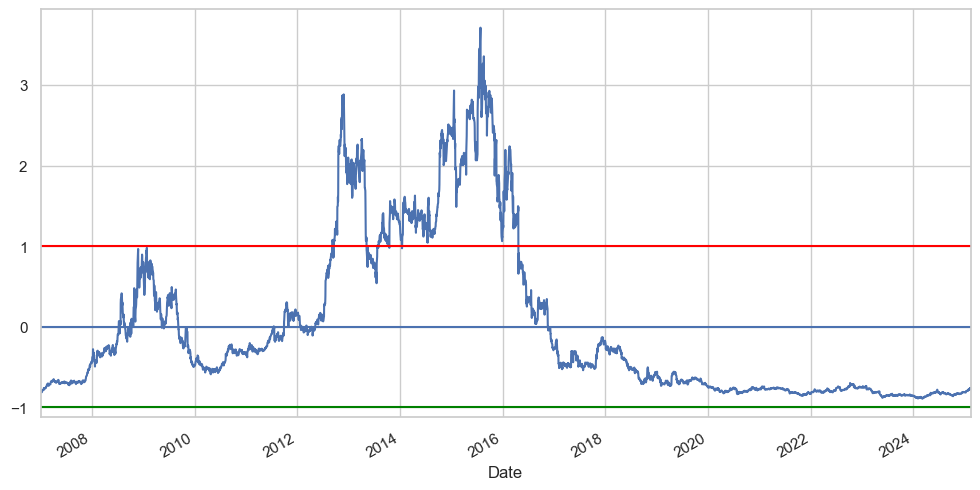
\includegraphics[width=0.8\linewidth]{plots/QCOM_AMD_ratio.png}
		\caption{Normalized Ratio between QCOM and AMD}
		\label{fig:qcom_amd_ratio}
	\end{figure}
\end{frame}

\begin{frame}
	\frametitle{ARCH/GARCH}
	
	\centering
	{\Large ARCH/GARCH Models}
\end{frame}

\begin{frame}{ARCH/GARCH}
	\begin{figure}[!h]
		\centering
		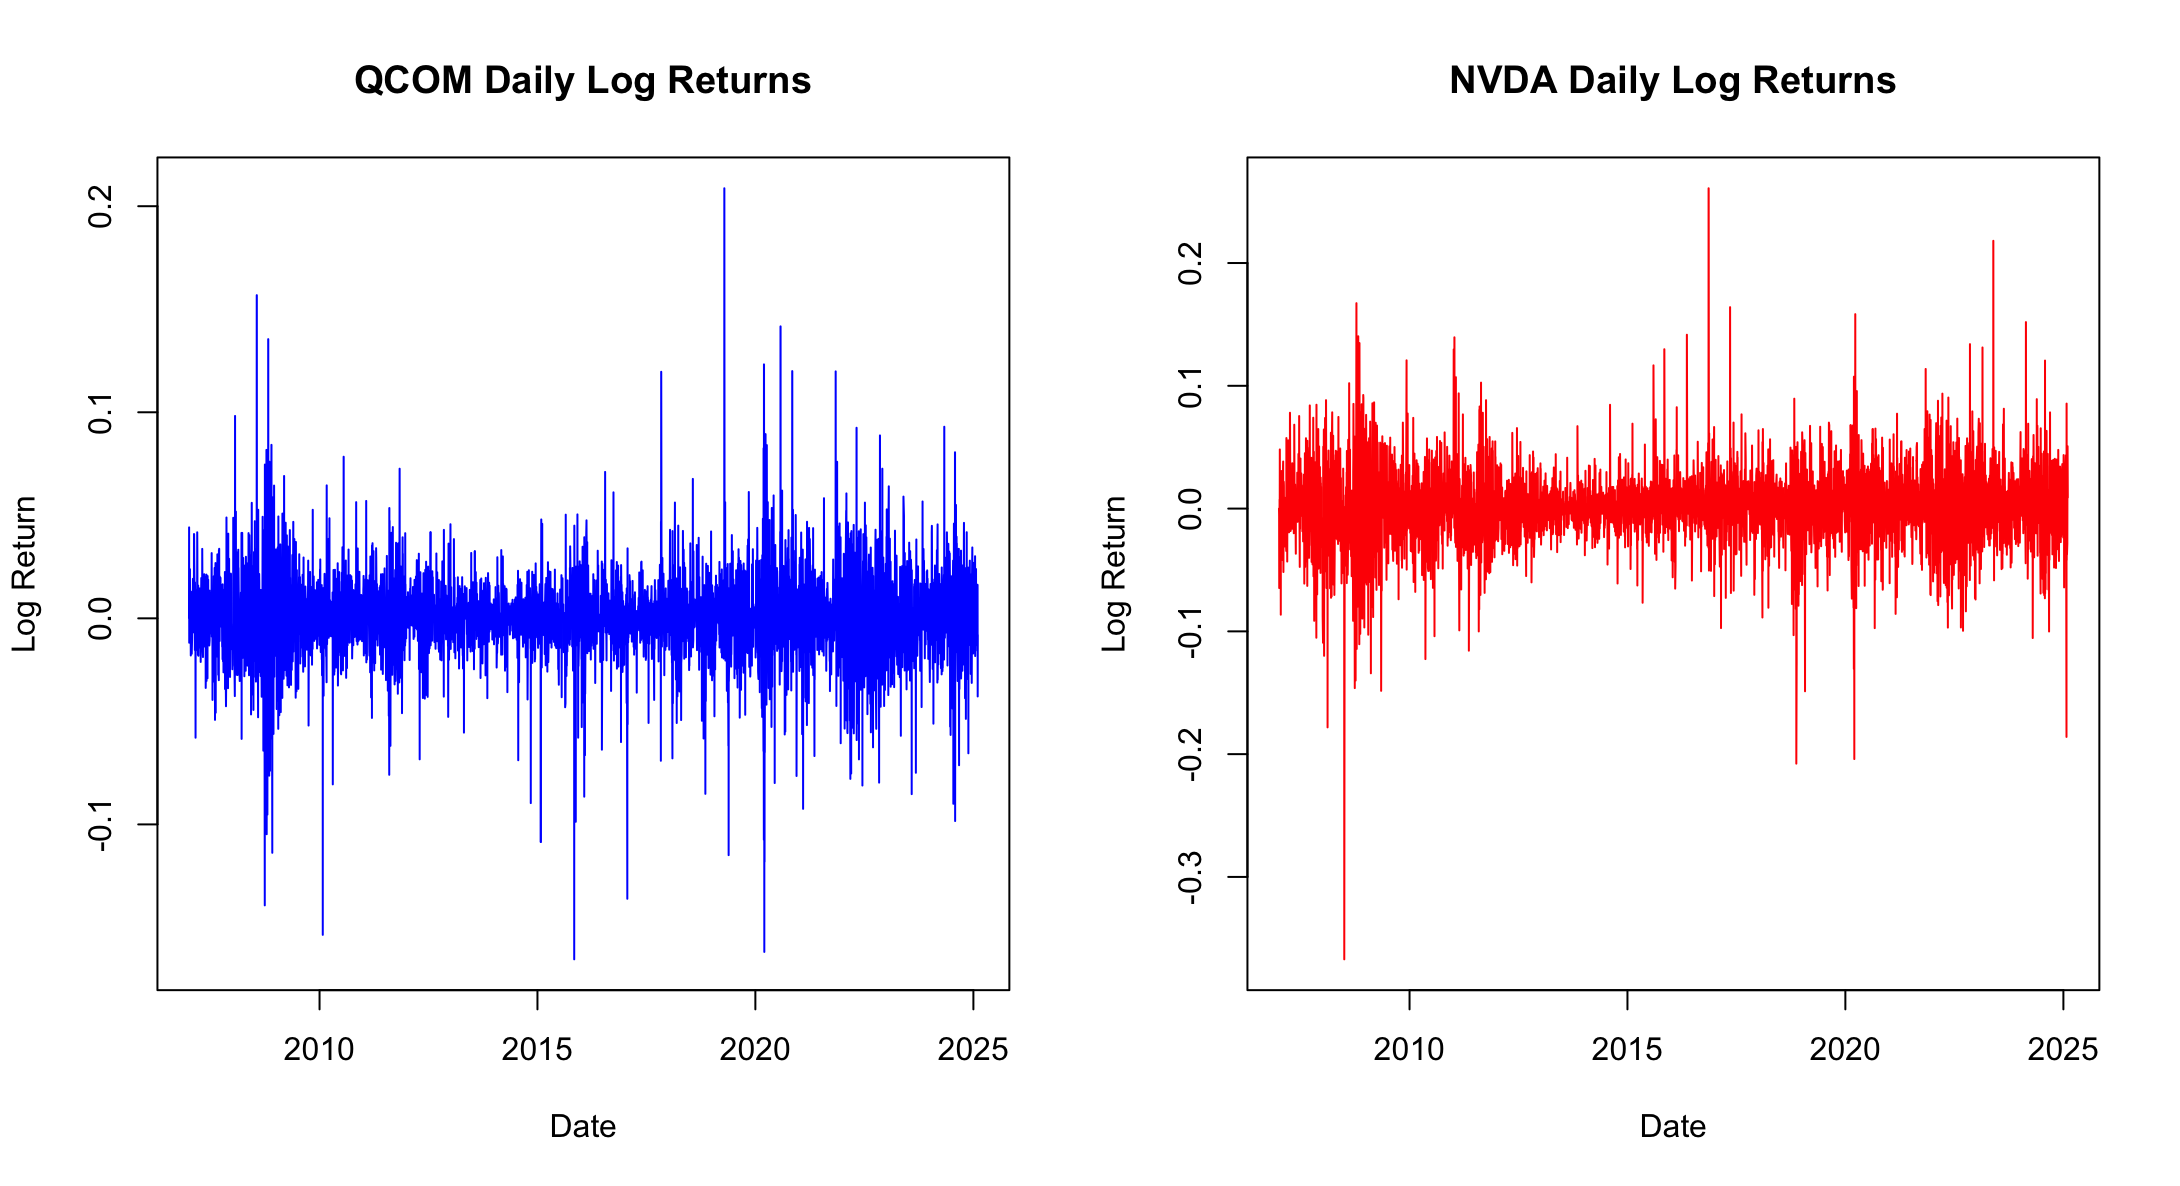
\includegraphics[width=0.8\linewidth]{plots/log_returns_QCOM_NVDA.png}
		\caption{Logged Returns for QCOM and NVDA}
	\end{figure}
\end{frame}

\begin{frame}{ARCH/GARCH}
	The ARCH/GARCH model has the following hypothesis test
	\newline
	\textbf{Hypothesis Test}
	\begin{itemize}
		\item $H_0: \rho_1(r^2)=\rho_2(r^2)=\dots\rho_m(r^2)=0$ 
		\item $H_a:\rho_j(r^2)\neq 0$ for at least one $j\in 1,2,\ldots,m$
	\end{itemize}
	\par
	\textbf{Test Statistic}
	\newline
	The Ljung-Box Q-statistic is defined as:
		\[
		\mathcal{Q}(m)=T(T+2)\sum_{j=1}^{m}\frac{\hat{\rho}_j^2}{T-j}
		\]
		
	Where
	\begin{itemize}
		\item $T$ is the sample size
		\item $m$ is the number of lags being tested
		\item $\hat{\rho}_j(r^2)$ is the sample autocorrelation of squared residuals at lag $j$
	\end{itemize}
\end{frame}

\begin{frame}{ARCH/GARCH}
	Under the null hypothesis, the test statistic 
	\[
	\mathcal{Q}(m)\sim\mathcal{X}^2(m-p-q)
	\]
	Where $p$ and $q$ represent the number of parameter in the fitted model (excluding constants and variance).
	\newline
	\textbf{Decision Rule:}
	\begin{itemize}
		\item Reject $H_0$ if $\mathcal{Q}(m)>\mathcal{X}^2_{\alpha, m-p-q}$
		\item Fail to reject $H_0$ if $\mathcal{Q}(m)\leq \mathcal{X}^2_{\alpha, m-p-q}$
	\end{itemize}
	where $ \mathcal{X}^2_{\alpha, m-p-q}$ is the critical value from the chi-square distribution with $m-p-q$ degrees of freedom at a siginficance level $\alpha$
\end{frame}

\begin{frame}{ARCH}
	\begin{figure}[!h]
		\centering
		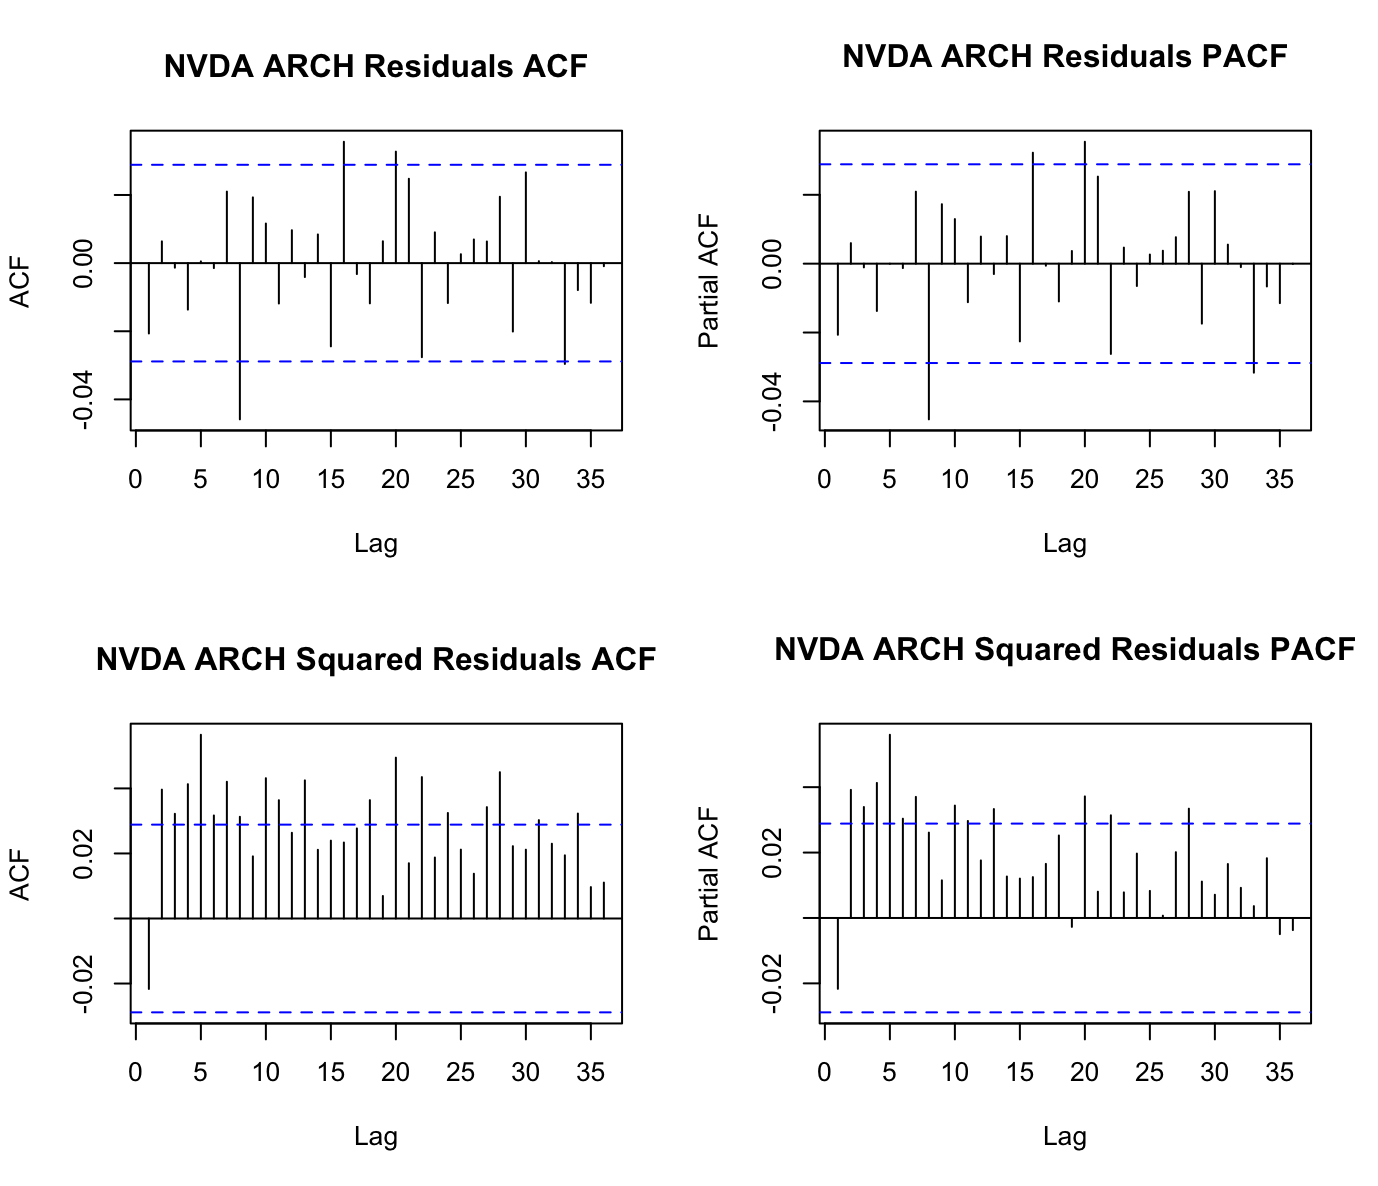
\includegraphics[width=0.65\linewidth]{plots/ARCH_NVDA.png}
		\caption{ACF and PACF for the Residual and Squared Residuals of NVDA}
	\end{figure}
\end{frame}

\begin{frame}{ARCH}
	\begin{figure}[!h]
		\centering
		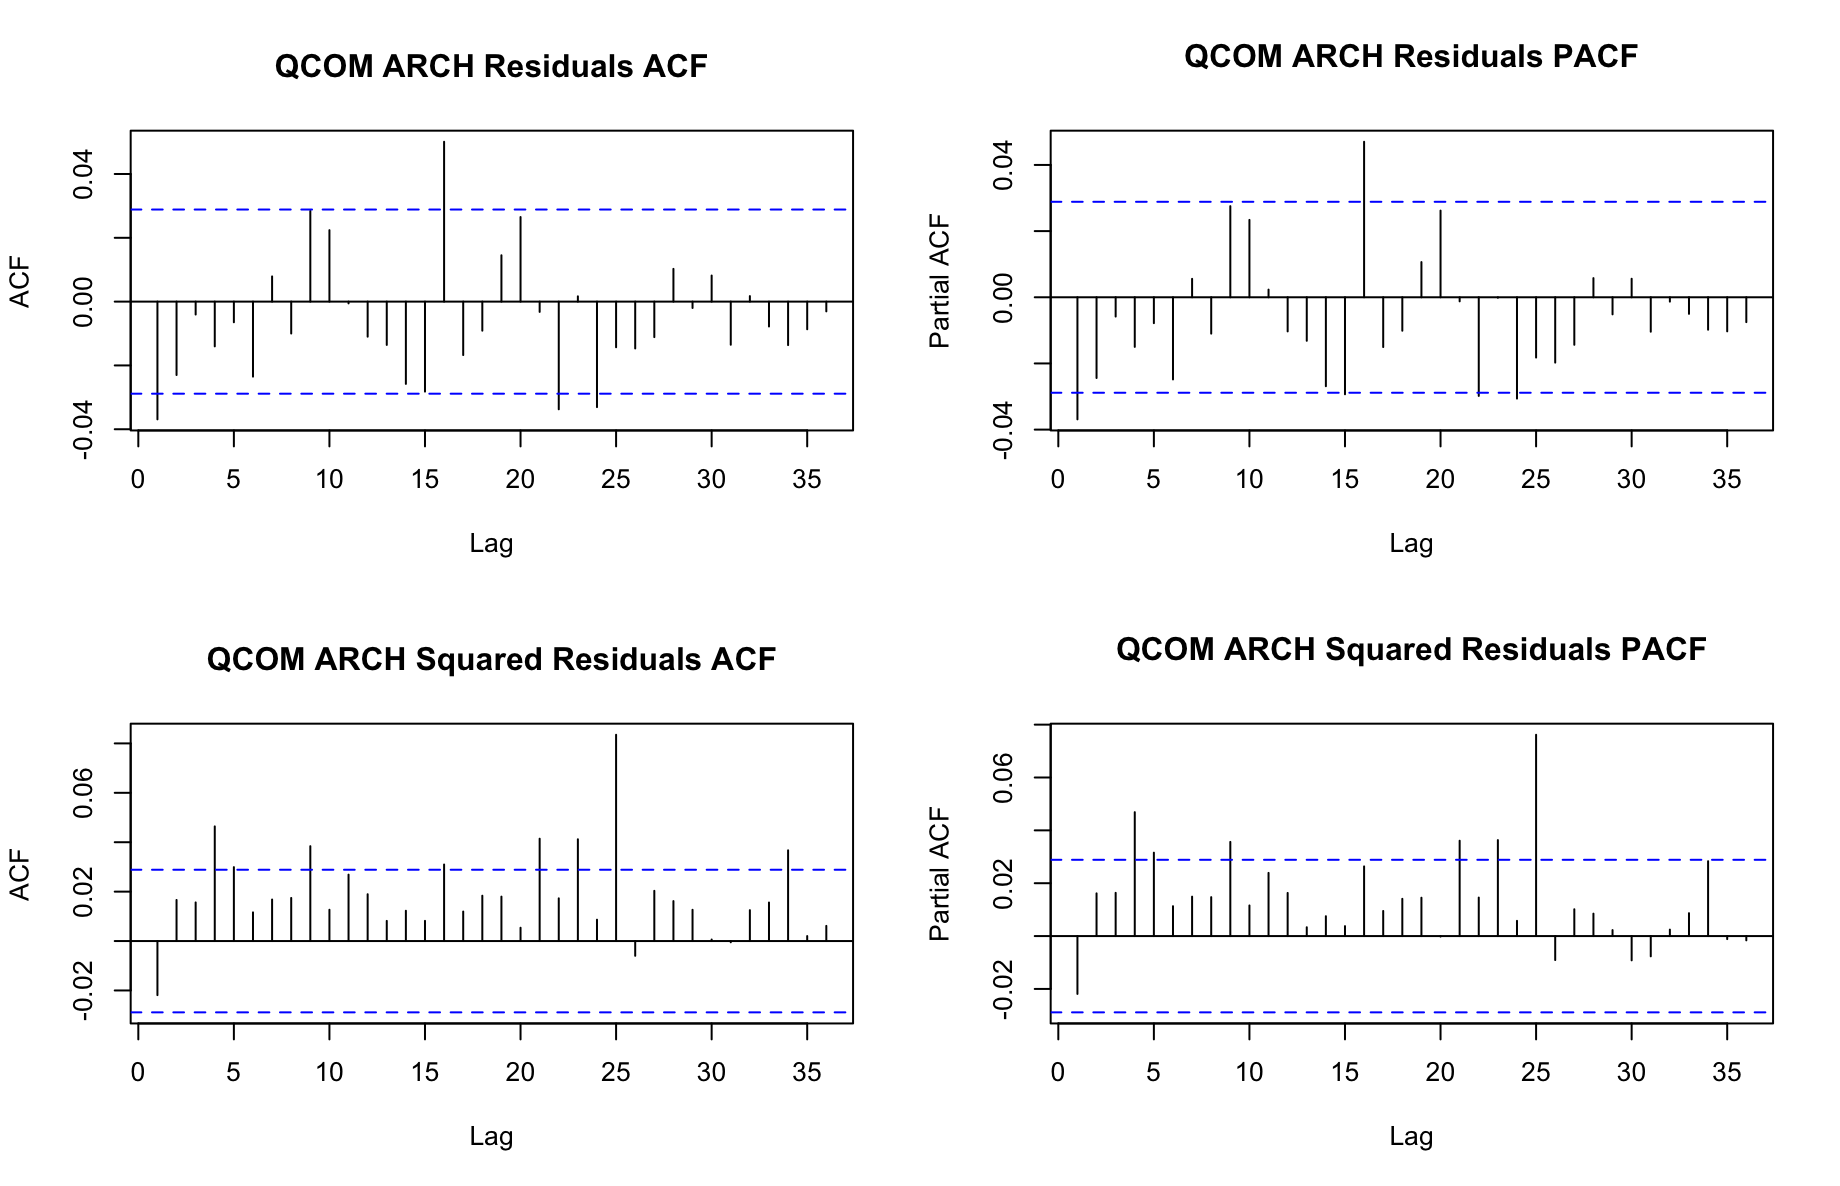
\includegraphics[width=0.8\linewidth]{plots/ARCH_QCOM.png}
		\caption{ACF and PACF for the Residual and Squared Residuals of QCOM}
	\end{figure}
\end{frame}

\begin{frame}{ARCH}
	\textbf{Conclusion: NVDA ARCH Model}
	\begin{enumerate}
		\item The ARCH model appears inadequate for capturing the full dynamics of NVDA’s return series:
		\begin{itemize}
			\item The significant autocorrelations in regular residuals indicate remaining serial correlation.
			\item The numerous significant spikes in squared residuals suggest unmodeled volatility dynamics.
		\end{itemize}
		\item Model improvements to consider:
		\begin{itemize}
			\item A higher-order ARCH model might help, but the extensive significant lags suggest a more fundamental issue.
			\item A GARCH model would likely be more appropriate, as it can better capture the persistence in volatility.
			\item Given the complex pattern of significant lags, more sophisticated models like EGARCH or GJR-GARCH might be worth exploring, especially if there are asymmetric volatility responses.
		\end{itemize}
	\end{enumerate}
\end{frame}

\begin{frame}{ARCH}
	\textbf{Conclusion: QCOM ARCH Model}
	\begin{enumerate}
		\item The ARCH model for QCOM shows moderate adequancy in modeling volatility but has clear limitations:
		\begin{itemize}
			\item The significant spikes in the residuals ACF/PACF indicate that the mean equation isn’t fully capturing the return dynamics.
			\item The significant spike at lag 25 in the squared residuals suggests specific periodicity in volatility that wasn’t modeled.
		\end{itemize}
		\item Model improvement suggestions:
		\begin{itemize}
			\item The mean equation specification should be revisited to better account for the serial correlation.
			\item A GARCH model would likely be more appropriate than the simple ARCH to capture the volatility persistence.
		\end{itemize}
	\end{enumerate}
\end{frame}

\begin{frame}{GARCH}
		\begin{figure}[!h]
		\centering
		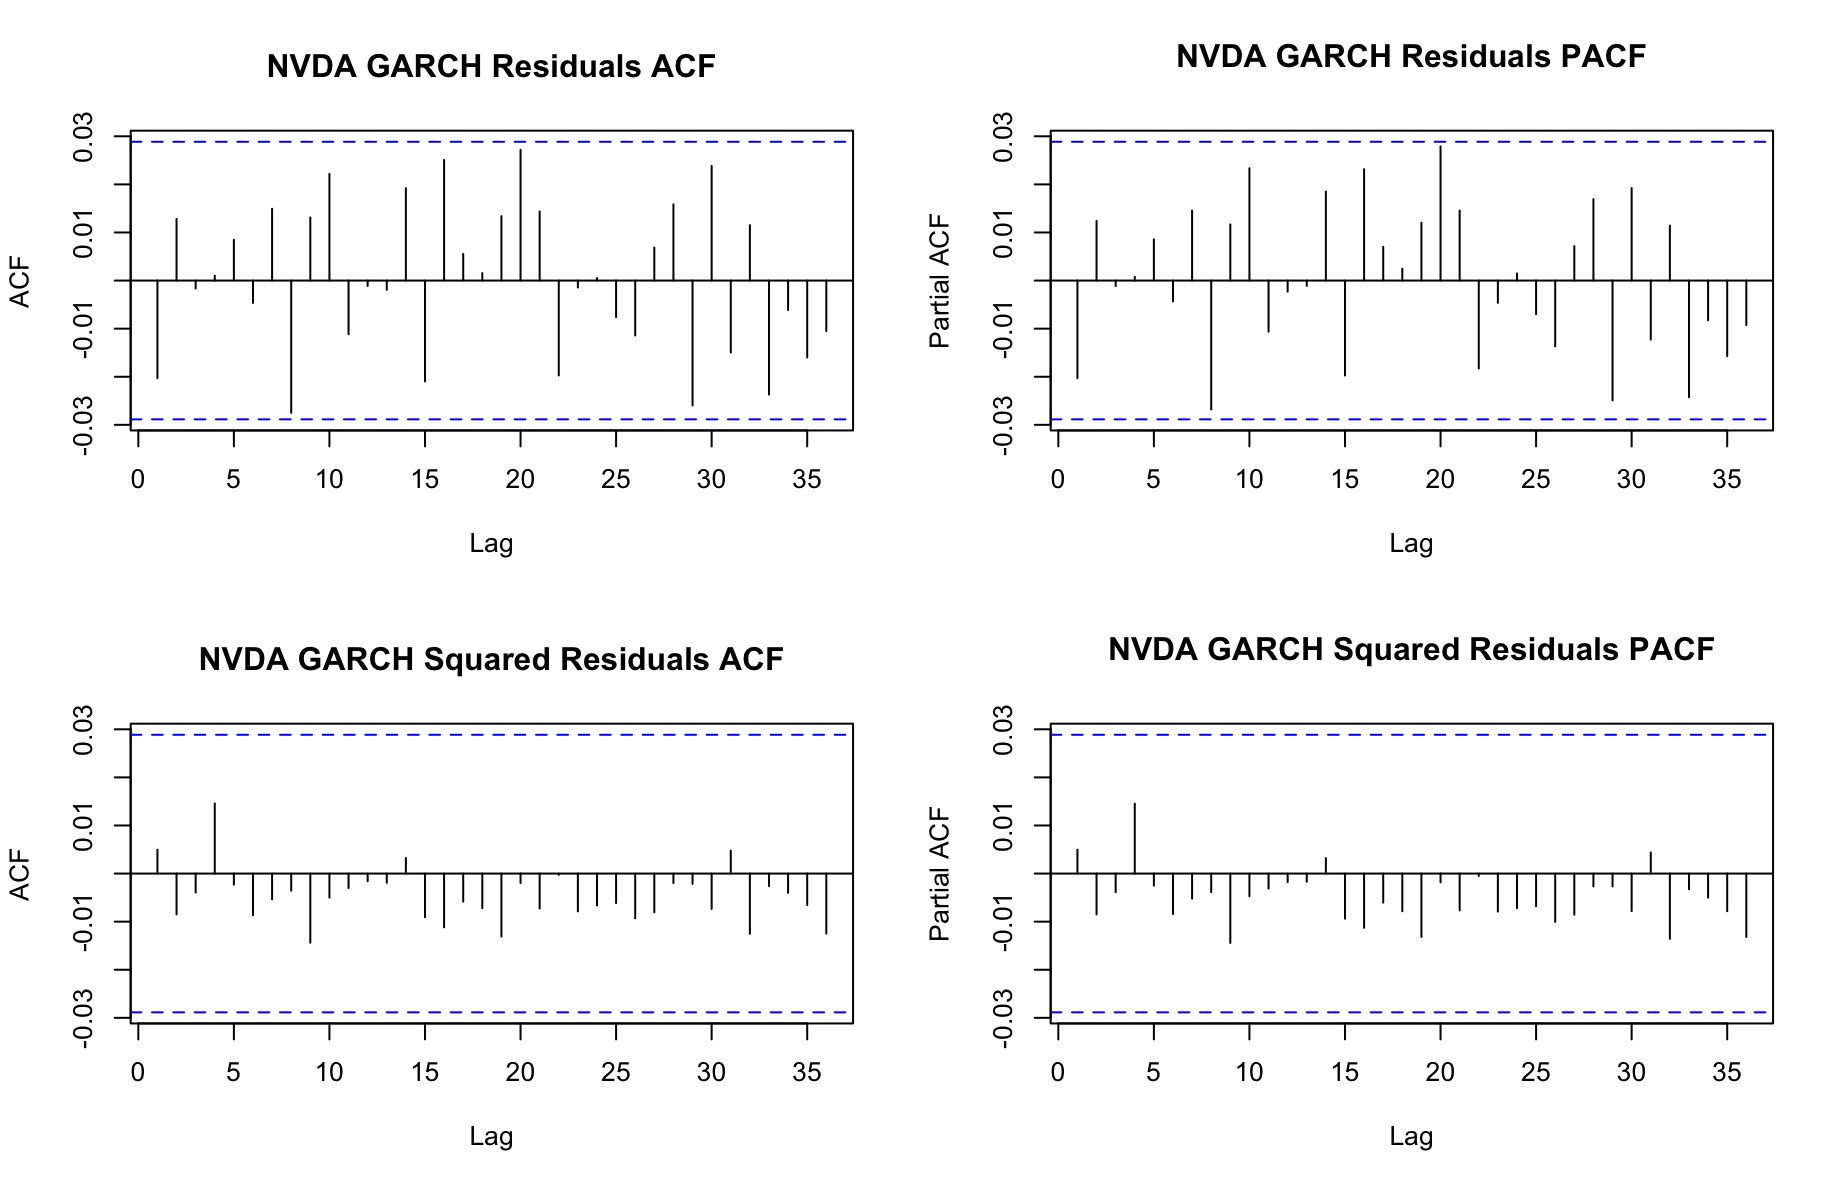
\includegraphics[width=0.65\linewidth]{plots/GARCH_NVDA.png}
		\caption{ACF and PACF for the Residual and Squared Residuals of NVDA}
	\end{figure}
\end{frame}

\begin{frame}{GARCH}
	\begin{figure}[!h]
		\centering
		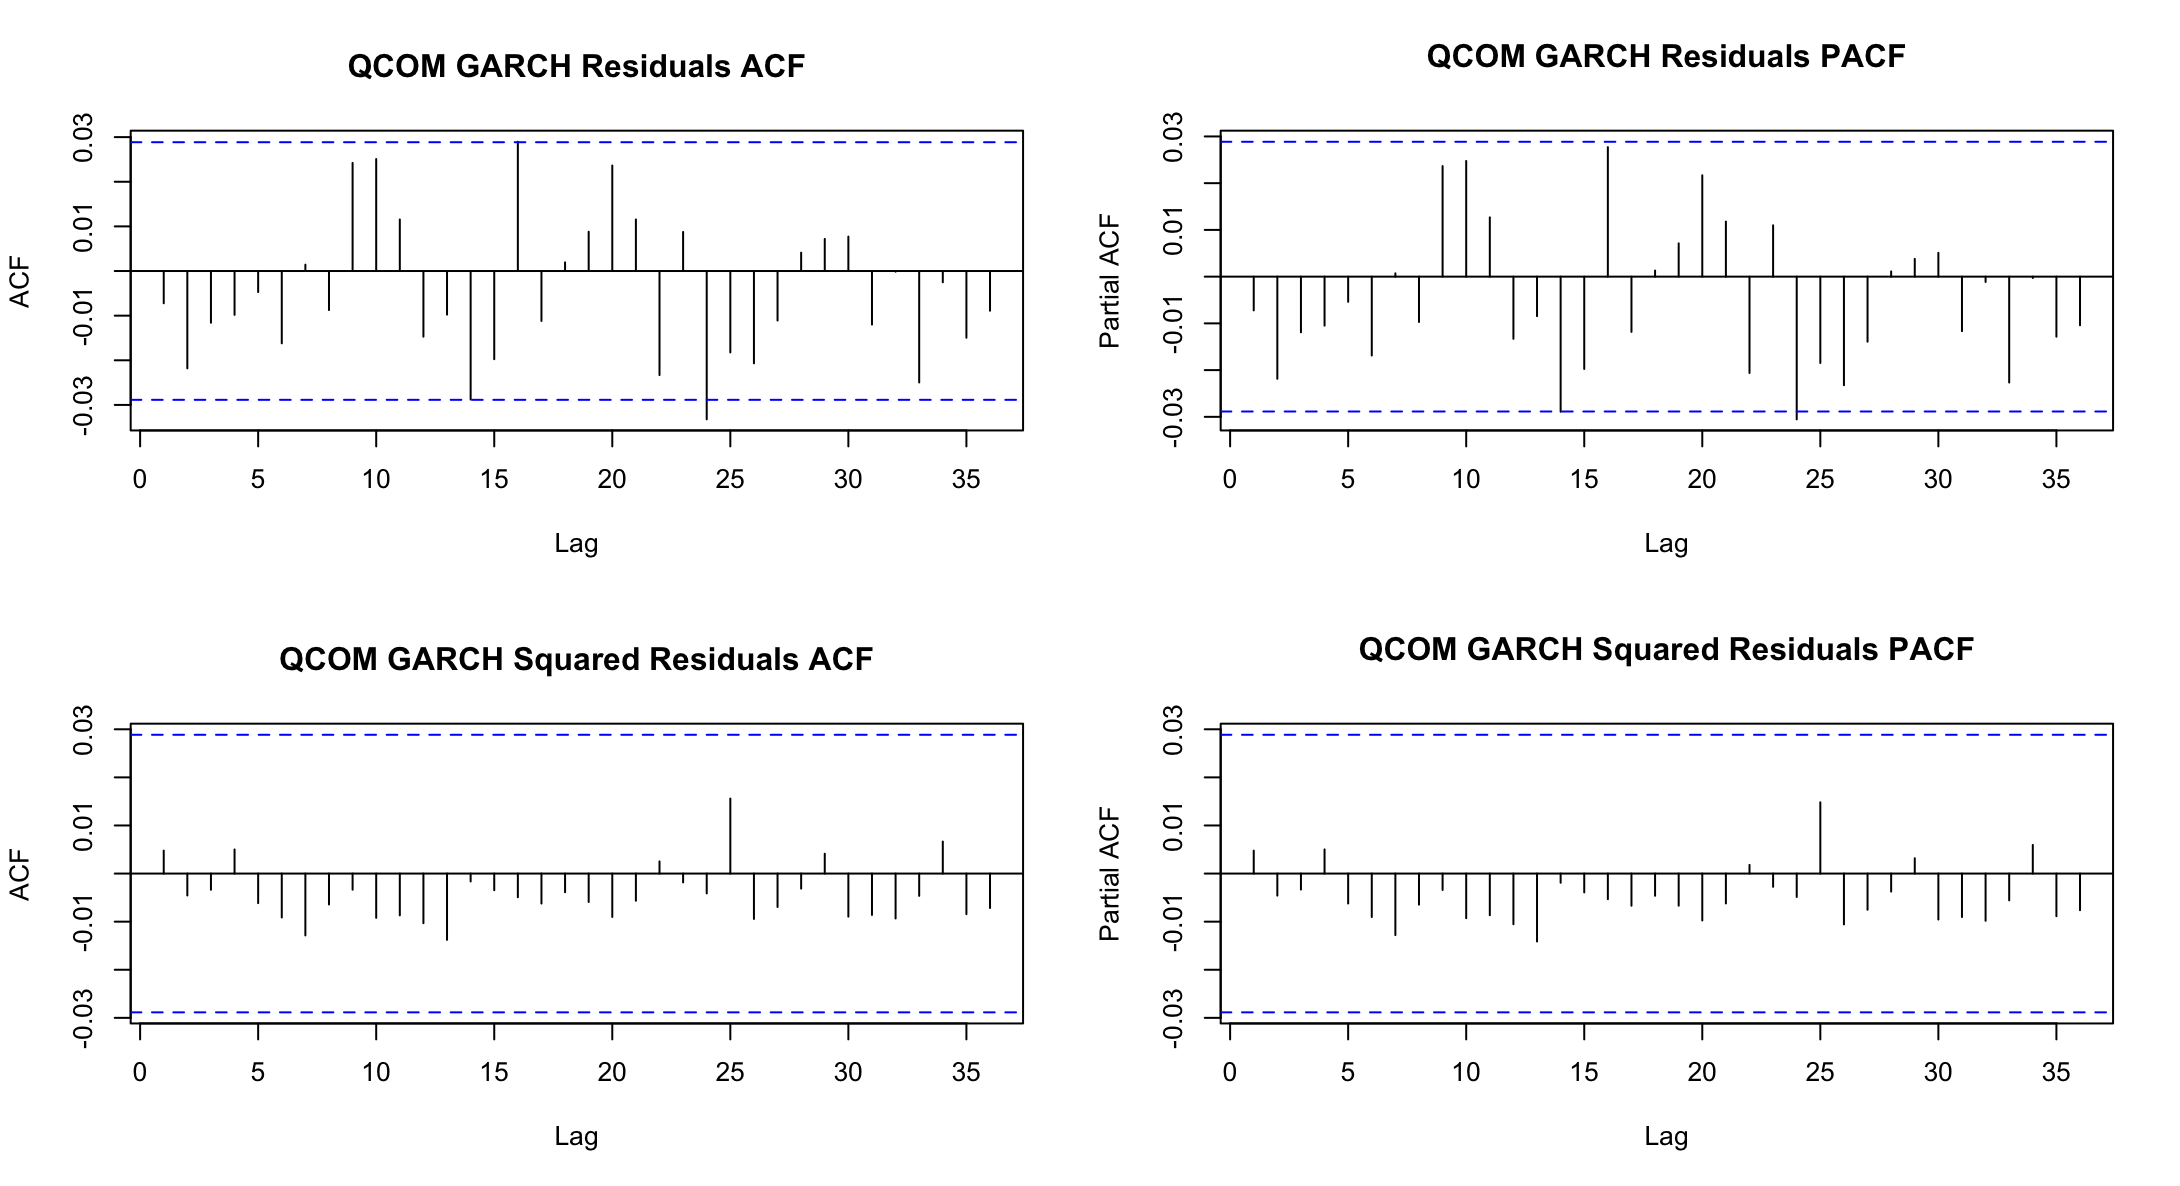
\includegraphics[width=0.8\linewidth]{plots/GARCH_QCOM.png}
		\caption{ACF and PACF for the Residual and Squared Residuals of QCOM}
	\end{figure}
\end{frame}

\begin{frame}{GARCH}
	\textbf{Conclusion: NVDA GARCH Model}
	\begin{enumerate}
		\item The GARCH model has done a reasonably good job capturing the volatility dynamics in NVDA returns, as evidenced by the lack of significant autocorrelation in squared residuals.
		\item There may be some minor remaining serial correlation in the standardized residuals, which suggests the mean equation might benefit from slight refinement.
		\item The absence of significant ARCH effects in the squared residuals indicates that the variance equation of the GARCH model is adequately specified.
	\end{enumerate}
\end{frame}

\begin{frame}{GARCH}
	\textbf{Conclusion: QCOM GARCH Model}
	\begin{enumerate}
	\item The GARCH model for QCOM has performed reasonably well in modeling the volatility dynamics:
	\begin{itemize}
		\item The squared residuals show very few significant autocorrelations, indicating successful modeling of volatility clustering.
		\item The single spike at lag 25 in the squared residuals might indicate some periodic pattern in volatility that occurs at that specific lag.
	\end{itemize}
	\item The mean equation specification could potentially be improved:
	\begin{itemize}
		\item The presence of several significant spikes in the residuals’ ACF and PACF suggests that the return dynamics aren’t fully captured.
		\item This might indicate that additional explanatory variables or a different ARMA specification might be beneficial.
	\end{itemize}
\end{enumerate}
\end{frame}

\begin{frame}{ARCH/GARCH}
	\scriptsize
\begin{table}[h!]
	\centering
	\caption{Weighted Ljung-Box Test Results for NVDA ARCH(1) and GARCH(1,1)}
	\begin{tabular}{llccc}
		\hline
		\textbf{Model} & \textbf{Residual Type} & \textbf{Lag} & \textbf{Statistic} & \textbf{$p$-value} \\
		\hline
		ARCH(1)   & Standardized Residuals      & Lag[1]              & 1.969   & 0.1606 \\
		&                             & Lag$(2(p+q)+(p+q)-1)$ & 2.063   & 0.2526 \\
		&                             & Lag$(4(p+q)+(p+q)-1)$ & 2.468   & 0.5126 \\
		& Squared Residuals           & Lag$(1)$              & 2.166   & 0.1411 \\
		&                             & Lag$(2(p+q)+(p+q)-1)$ & 5.790   & 0.0250 \\
		&                             & Lag$(4(p+q)+(p+q)-1)$ & 16.934  & 0.0001 \\
		GARCH(1,1) & Standardized Residuals     & Lag[1]              & 1.905   & 0.1676 \\
		&                            & Lag$(2(p+q)+(p+q)-1)$ & 2.284   & 0.2197 \\
		&                            & Lag$(4(p+q)+(p+q)-1)$ & 2.587   & 0.4875 \\
		& Squared Residuals          & Lag$(1)$              & 0.114   & 0.7352 \\
		&                            & Lag$(2(p+q)+(p+q)-1)$ & 0.820   & 0.8989 \\
		&                            & Lag$(4(p+q)+(p+q)-1)$ & 1.450   & 0.9596 \\
		\hline
	\end{tabular}
	\label{tab:nvda_combined_wlb}
\end{table}
\end{frame}
\begin{frame}
	\frametitle{Value-at-Risk}
	
	\centering
	{\Large Value-at-Risk}
\end{frame}

\begin{frame}{Value-at-Risk: Introduction}
	\begin{itemize}
		\item Value at Risk (VaR) measures the maximum potential loss over a given time at a certain confidence level.
		\item Assets analyzed: \textbf{QCOM} and \textbf{NVDA}
		\item 1-day VaR computed at 95\% and 99\% confidence levels
		\item Methods used:
		\begin{itemize}
			\item Historical VaR
			\item Parametric (Gaussian) VaR
			\item GARCH-Based VaR
		\end{itemize}
	\end{itemize}
\end{frame}

\begin{frame}{Historical VaR – Methodology}
	\begin{itemize}
		\item Non-parametric method: directly uses the empirical distribution of past returns.
		\item Sort log returns from smallest to largest.
		\item Select the quantile corresponding to the desired confidence level:
		\[
		\text{VaR}_{\alpha} = \text{Quantile}_{(1 - \alpha)}(\text{Returns})
		\]
		\item Example: 5th percentile of NVDA’s historical daily returns gives the 95\% 1-day VaR.
		\item \textbf{Assumption}: Past return distribution approximates future risk.
	\end{itemize}
\end{frame}

\begin{frame}{Historical VaR – NVDA vs QCOM (95\%)}
	\begin{figure}[!h]
		\centering
		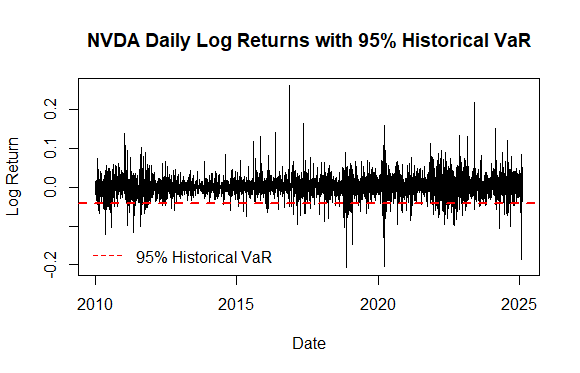
\includegraphics[width=0.45\textwidth]{plots/nvda_hist_var_plot.png}
		\hspace{0.05\textwidth}
		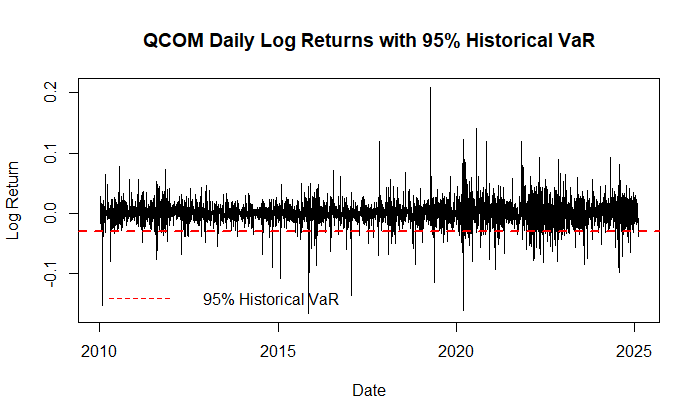
\includegraphics[width=0.45\textwidth]{plots/qcom_hist_var_plot.png}
		\caption{NVDA and QCOM Daily Log Returns with 95\% Historical VaR}
	\end{figure}
\end{frame}

\begin{frame}{VaR Violations – NVDA (95\%)}
	\begin{figure}[!h]
		\centering
		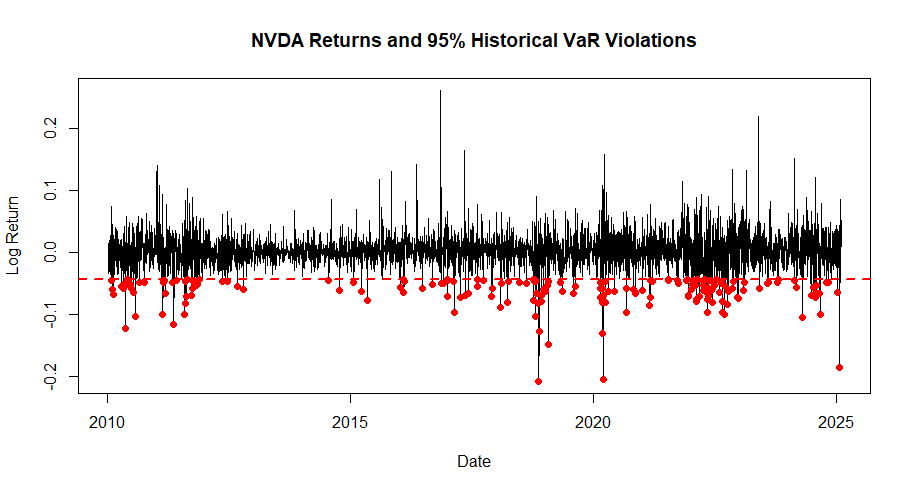
\includegraphics[width=0.85\textwidth]{plots/nvda_hist_var_marked.png}
		\caption{Daily Log Returns of NVDA with 95\% Historical VaR and Violation Points}
	\end{figure}
\end{frame}

\begin{frame}{VaR Violations – QCOM (95\%)}
	\begin{figure}[!h]
		\centering
		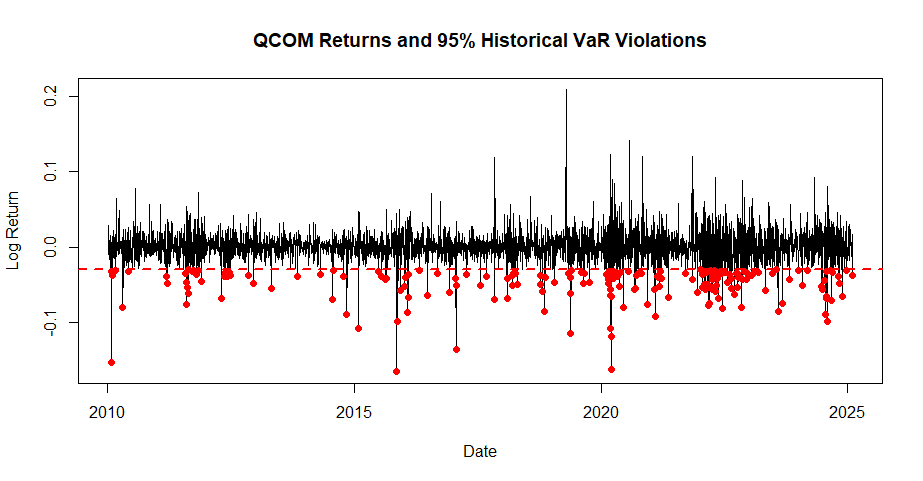
\includegraphics[width=0.85\textwidth]{plots/qcom_hist_var_marked.png}
		\caption{Daily Log Returns of QCOM with 95\% Historical VaR and Violation Points}
	\end{figure}
\end{frame}

\begin{frame}
	\frametitle{From Historical to Parametric VaR}
	\centering
	\Large
	Historical VaR assumes the past will repeat...  
	But what if we believe returns follow a known distribution?
\end{frame}

\begin{frame}{Parametric VaR – Gaussian Assumption}
	\begin{itemize}
		\item Assumes returns are normally distributed with mean $\mu$ and standard deviation $\sigma$.
		\item VaR formula:
		\[
		\text{VaR}_\alpha = \mu - z_\alpha \cdot \sigma
		\]
		where $z_\alpha$ is the z-score for confidence level $\alpha$ (e.g., 1.645 for 95\%).
		\item \textbf{Advantage}: Quick to compute.
		\item \textbf{Limitation}: May underestimate tail risk due to normality assumption.
	\end{itemize}
\end{frame}

\begin{frame}{Parametric VaR – NVDA}
	\begin{figure}[!h]
		\centering
		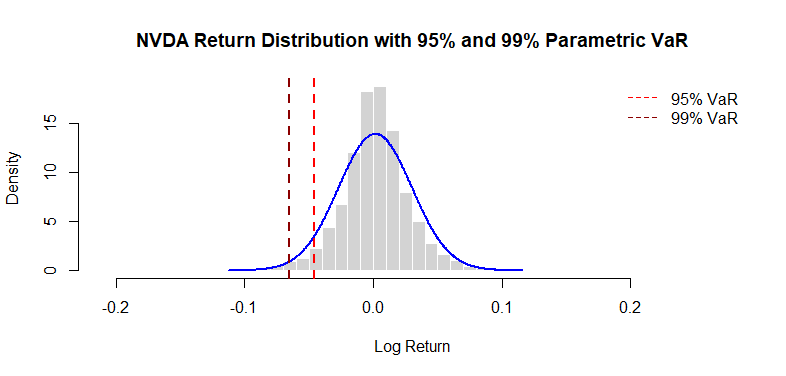
\includegraphics[width=0.85\textwidth]{plots/nvda_parametric_var_hist.png}
		\caption{NVDA Return Distribution with 95\% and 99\% Parametric VaR Cutoffs}
	\end{figure}
\end{frame}

\begin{frame}{Parametric VaR – QCOM}
	\begin{figure}[!h]
		\centering
		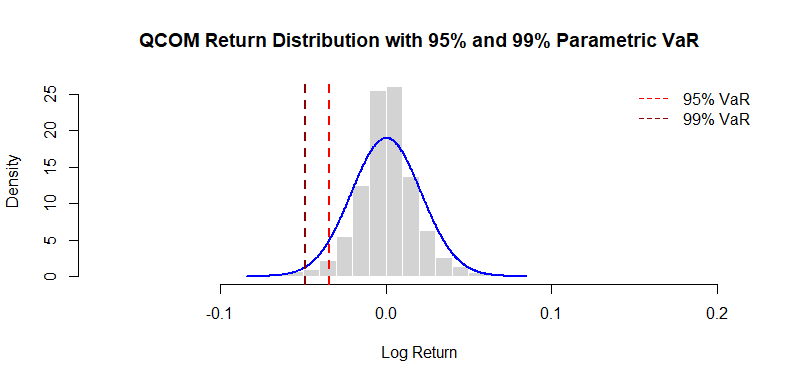
\includegraphics[width=0.85\textwidth]{plots/qcom_parametric_var_hist.png}
		\caption{QCOM Return Distribution with 95\% and 99\% Parametric VaR Cutoffs}
	\end{figure}
\end{frame}

\begin{frame}{Empirical vs Theoretical Gaussian – NVDA}
	\begin{figure}[!h]
		\centering
		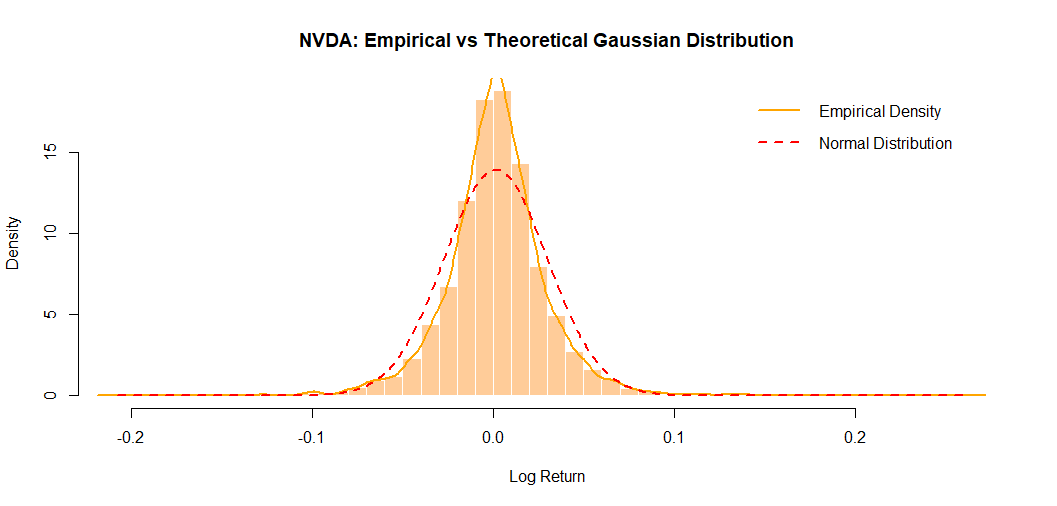
\includegraphics[width=0.85\linewidth]{plots/nvda_density_plot.png}
		\caption{NVDA: Empirical Return Density vs. Normal Distribution}
	\end{figure}
\end{frame}

\begin{frame}{Empirical vs Theoretical Gaussian – QCOM}
	\begin{figure}[!h]
		\centering
		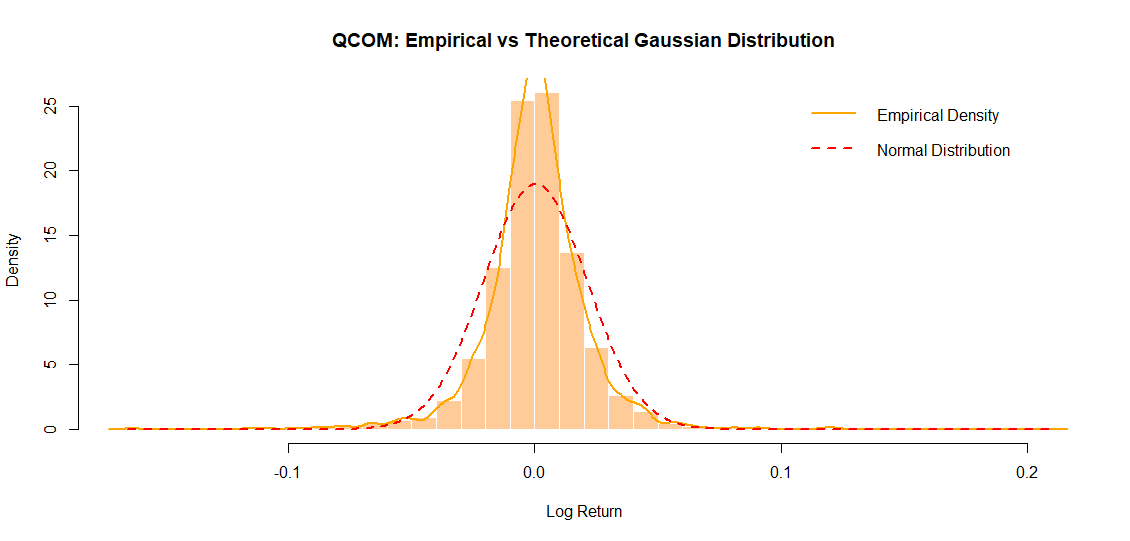
\includegraphics[width=0.85\linewidth]{plots/qcom_density_plot.png}
		\caption{QCOM: Empirical Return Density vs. Normal Distribution}
	\end{figure}
\end{frame}


\begin{frame}
	\frametitle{From Parametric to GARCH-Based VaR}
	\centering
	\Large
	Parametric VaR assumes constant volatility... \\
	But markets often exhibit volatility clustering. \\
	Can we model that dynamically?
\end{frame}

\begin{frame}{GARCH-Based VaR – Motivation}
	\begin{itemize}
		\item Financial time series often exhibit:
		\begin{itemize}
			\item Volatility clustering
			\item Heavy tails
		\end{itemize}
		\item GARCH(1,1) models allow volatility to change over time:
		\[
		\sigma_t^2 = \omega + \alpha \epsilon_{t-1}^2 + \beta \sigma_{t-1}^2
		\]
		\item We forecast next-period $\mu_t$ and $\sigma_t$, then apply:
		\[
		\text{VaR}_\alpha = \mu_t - z_\alpha \cdot \sigma_t
		\]
		\item More responsive to recent market conditions.
	\end{itemize}
\end{frame}

\begin{frame}{GARCH Conditional Volatility – NVDA vs QCOM}
	\textbf{Volatility Forecast }
	\begin{figure}[!h]
		\centering
		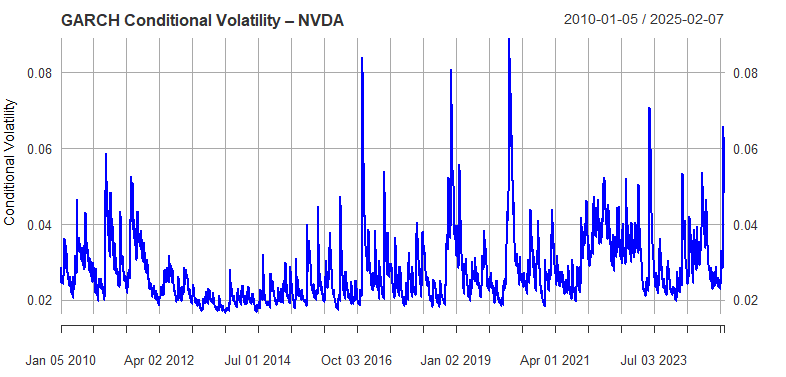
\includegraphics[width=0.45\textwidth]{plots/nvda_garch_vol.png}
		\hspace{0.05\textwidth}
		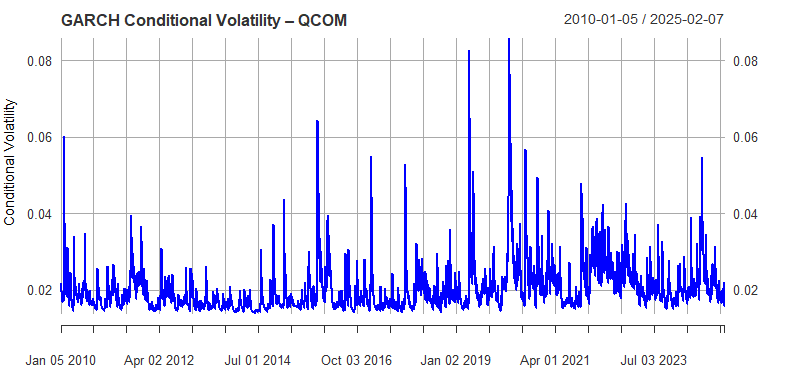
\includegraphics[width=0.45\textwidth]{plots/qcom_garch_vol.png}
		\caption{Time-Varying Volatility from GARCH(1,1) Models for NVDA and QCOM}
	\end{figure}
\end{frame}

\begin{frame}{GARCH Conditional Volatility – NVDA}
	\textbf{Volatility Forecast}
	\begin{figure}[!h]
		\centering
		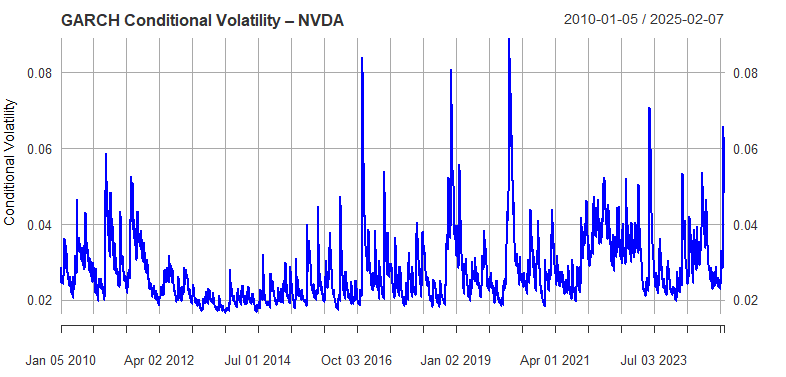
\includegraphics[width=0.85\linewidth]{plots/nvda_garch_vol.png}
		\caption{Time-Varying Conditional Volatility from GARCH(1,1) Model for NVDA}
	\end{figure}
\end{frame}

\begin{frame}{GARCH Conditional Volatility – QCOM}
	\textbf{Volatility Forecast}
	\begin{figure}[!h]
		\centering
		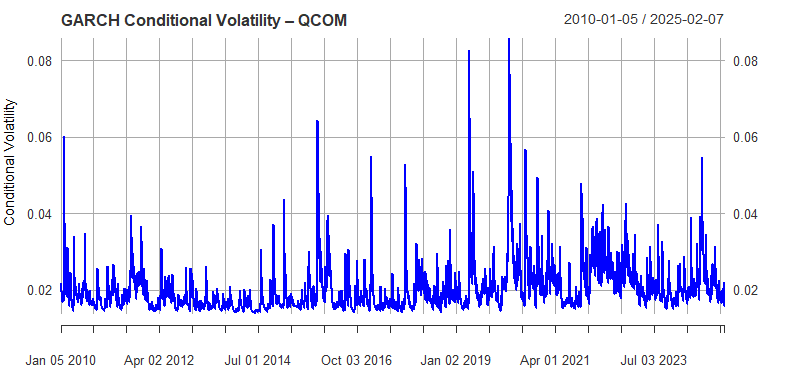
\includegraphics[width=0.85\linewidth]{plots/qcom_garch_vol.png}
		\caption{Time-Varying Conditional Volatility from GARCH(1,1) Model for QCOM}
	\end{figure}
\end{frame}


\begin{frame}{VaR Estimates – Summary Table}
	\textbf{VaR Estimates Summary }
	\centering
	\begin{tabular}{lccc}
		\toprule
		\textbf{Method} & \textbf{VaR Level} & \textbf{NVDA} & \textbf{QCOM} \\
		\midrule
		Historical       & 95\%  & -4.29\%  & -3.01\% \\
		& 99\%  & -7.30\%  & -6.38\% \\
		Parametric       & 95\%  & -4.56\%  & -3.43\% \\
		(Gaussian)       & 99\%  & -6.51\%  & -4.86\% \\
		GARCH-Based      & 95\%  & -7.73\%  & -3.59\% \\
		& 99\%  & -11.01\% & -5.09\% \\
		\bottomrule
	\end{tabular}
\end{frame}

\begin{frame}{Interpreting the VaR Estimates Summary}
	\begin{itemize}
		\item \textbf{Historical VaR:} 
		\begin{itemize}
			\item Reflects empirical tail behavior.
			\item NVDA shows higher loss potential than QCOM.
		\end{itemize}
		
		\item \textbf{Parametric (Gaussian) VaR:}
		\begin{itemize}
			\item Easier to compute but underestimates tail risk.
			\item 99\% VaR for NVDA is notably less negative than Historical.
		\end{itemize}
		
		\item \textbf{GARCH-Based VaR:}
		\begin{itemize}
			\item Captures time-varying volatility.
			\item Produces the most conservative estimates, especially for NVDA.
			\item Better suited for assets with volatility clustering.
		\end{itemize}
		
		\item \textbf{Conclusion:}
		\begin{itemize}
			\item GARCH offers superior risk estimation for tech stocks like NVDA.
			\item Method choice significantly affects perceived risk.
		\end{itemize}
	\end{itemize}
\end{frame}

\begin{frame}
	\frametitle{Beyond VaR: Introducing Expected Shortfall (ES)}
	\centering
	\Large
	Value-at-Risk tells us the minimum loss in the worst-case...\\[1em]
	\textbf{But what happens if things get even worse?} \\[2em]
	\normalsize
	Expected Shortfall helps us answer that.
\end{frame}


\begin{frame}{Expected Shortfall (95\%) – Parametric}
	\textbf{Expected Shortfall: A Deeper Risk Measure}
	\begin{itemize}
		\item While VaR tells us the threshold of loss, Expected Shortfall (ES) tells us how bad it can get beyond that threshold.
		\item \textbf{NVDA}: -5.76\%
		\item \textbf{QCOM}: -4.30\%
		\item ES is a coherent risk measure that better captures tail risk than VaR.
	\end{itemize}
\end{frame}

\begin{frame}{Comparison of VaR Methods}
	\textbf{Comparison of all three VaR Methods}
	\tiny
	\renewcommand{\arraystretch}{1.4}  % Adjust row spacing
	\begin{tabularx}{\textwidth}{l|X|X|X}
		\toprule
		\textbf{Feature} & \textbf{Historical VaR} & \textbf{Parametric VaR} & \textbf{GARCH-Based VaR} \\
		\midrule
		Model Assumption & None (empirical returns) & Normal distribution & Time-varying volatility \\
		\midrule
		Tail Sensitivity & Captures empirical tails & Often underestimates & Captures volatility clustering \\
		\midrule
		Ease of Computation & Simple & Very fast & Moderate (needs estimation) \\
		\midrule
		Volatility Assumption & Constant over time & Constant over time & Dynamic \\
		\midrule
		Reactiveness to Market & Low & Low & High \\
		\midrule
		Common Use Case & Backtesting, benchmarking & Quick estimate & Trading, stress testing \\
		\bottomrule
	\end{tabularx}
\end{frame}

\begin{frame}{Key Takeaways}
	\begin{itemize}
		\item Time series models like VAR, ARCH, and GARCH help capture dynamics in financial data.
		\item VaR provides a standardized way to assess risk—each method has trade-offs.
		\item GARCH-Based VaR is more adaptive to market conditions but computationally intensive.
		\item Choosing the right model depends on context: simplicity vs. accuracy vs. responsiveness.
	\end{itemize}
\end{frame}

\begin{frame}{Applications in Practice}
	\begin{itemize}
		\item Risk management in trading desks and portfolio monitoring
		\item Stress testing and regulatory compliance (e.g., Basel III)
		\item Strategy development for hedge funds and market makers
		\item Useful in modeling volatility spillovers and financial contagion
	\end{itemize}
\end{frame}

\begin{frame}
	\centering
	\vspace{2cm}
	{\Huge \textbf{Thank You!}}\\[1em]
	{\Large Questions and Discussion Welcome}\\[2em]
	\textit{Andre Sealy, Federica Malamisura, Swapnil Pant}\\
	\textit{FA 542 – Time Series with Applications to Finance}\\
	\textit{Stevens Institute of Technology}
\end{frame}


\end{document}
